\chapter{Conclusions}\label{cap.conclusions}

 

In this thesis we studied deep learning techniques and their application in a tracking algorithm. We were able to build a tracking algorithm that utilizes a neural network and do not miss the real time objective. To do so we used the tracking-by-detection framework, it combines people detection using a neural network, somehow, slow but very accurate, and link these detections with feature tracking, very quick but prone to drift.  In addition we studied the person reidentification problem and we solved with a deep learning techniques.

Finally we evaluated our algorithm in a well-known challenge, MOT16, and analyses its performance and timing capabilities on it. The algorithms performs reasonably well in sequences of high frame rate and resolution, but in the opposite sequences, low frame rate and resolution the performance drop dramatically. This is happens because our algorithm rely on points with high texture, with a low resolution there are less points with this characteristics. Also, we have problems with people who wear low texture or are away from the camera, as we can observe in figure \ref{Fails1}. The low frame rate, penalize the matching capabilities between frames, it produces wrong matches between images, therefore, wrong displacements.




\begin{figure}[H]
		
\centering

\subfigure[High texture person.]{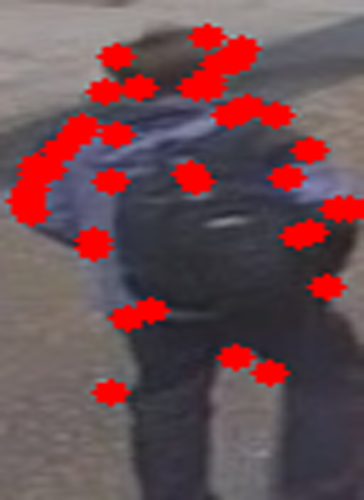
\includegraphics[width=3cm]{changeCamera/tomeuTetx.png}}
\subfigure[Low texture person.]{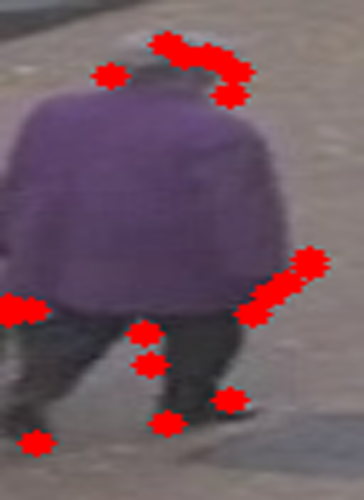
\includegraphics[width=3cm]{changeCamera/donaTetx.png}}
\subfigure[Far away person.]{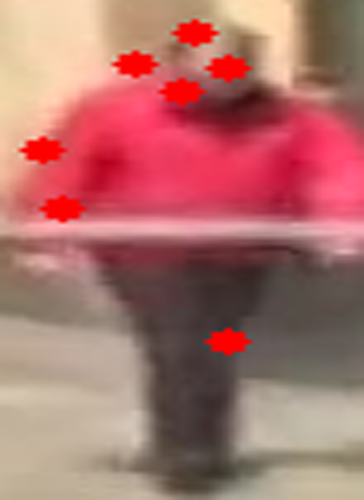
\includegraphics[width=3cm]{changeCamera/foto004.png}}
\caption{Differences texture examples.}
\label{Fails1}
\end{figure}








\section{Future work}


This is a first entrance on trackings algorithm, we have a reasonable results. We can add some details to improve our results.


\begin{itemize}

\item Port to C++. We used a srcipting programming languagge, if we switch to a compiled programing language we would increase the time perfomance.

\item GPU implementation. Computing displacement for each tracket could be computed in a parallel way. They are independent from each other and are a low demanding. 

\item Propbabilistic framework. Include bayesian filter techniques to increase perfomance.

\item Siamese architectures. Study new siamese architecture to increase the accuracy of this modeule, like inception stem of InceptionV3 or include the optical flow information in the neural network.

\item Data association. Use much confidence techniques to associate the detections, the current methods relay ond probablistic graphical models.

\end{itemize}
